\section{Auswertung}
Hier Allgemeines aufführen

\subsection{Bestimmung der Grenzfrequenzen aus den Durchlasskurven}
Um die Grenzfrequenzen aus dem Verlauf der Durchlasskurven zu ermitteln, wurden jeweils sechs
Frequenzen mit dem zugehörigen Abstand $x$ zum gewählten Nullpunkt aufgezeichnet. Die Messwerte
sind in Tabelle \ref{tab: sweep_LC} aufgeführt. Diese Referenzpunkte ermöglichen einen Fit an eine Funktion der Form:
\begin{equation}
  \nu(x) = A \cdot \exp(B\cdot x) + C
  \label{eq: exp_fit}
\end{equation}
\FloatBarrier
\begin{table} 
\centering 
\caption{LC-Kette, Referenzpunkte für den Frequenzsweep} 
\label{tab: sweep_LC} 
\begin{tabular}{S S } 
\toprule  
{x in $\si{\centi\meter}$} & {Frequenzen in $\si{\hertz}$}  \\ 
\midrule  
 0  & 25871\\ 
4  & 34357\\ 
8  & 44939\\ 
12  & 57992\\ 
16  & 74697\\ 
20  & 102876\\ 
\bottomrule 
\end{tabular} 
\end{table}
Für die LC-Kette ergeben sich folgende Parameter:
\begin{align}
  \begin{aligned}
    A\ua{LC} &= \SI{1.9(4)e4}{\hertz}\\
    B\ua{LC} &= \SI{0.079(8)}{\cm^{-1}}\\
    C\ua{LC} &= \SI{7(5)e3}{\hertz}
  \end{aligned}
  \label{eq: params_LC}
\end{align}
Die Messwerte, sowie der Verlauf des Fits sind in Abbildung \ref{fig: plot_sweep_LC} dargestellt. Zusammen
mit dem Abstand $x\ua{G} = \SI{10.2(5)}{cm}$, der auf dem Millimeterpapier abgelesen wurde, ergibt sich
für die Grenzfrequenz:
\begin{equation}
  \nu\ua{G, exp}\SI{5.1(11)e4}{\hertz}
  \label{eq: nu_g_LC}
\end{equation}
Der angegebene Fehler von $\SI{5}{\milli\meter}$ wurde gewählt, um Ableseungenauigkeiten und die in den Durchlasskurven
erkennbaren Störsignale zu berücksichtigen.
Mit Formel \eqref{eq: } und den Apparaturkonstanten ergibt sich der zugehörige theoretische Wert $\nu\ua{G, th}$, sowie die
mittlere prozentuale Abweichung $d\ua{LC}$ des experimentell bestimmten Wertes zu:
\begin{align}
  \nu\ua{G, th} &= \SI{5.13e4}{\hertz} \\
  d\ua{LC} &= 1 \%
\end{align}
\FloatBarrier
\begin{figure}
  \centering
  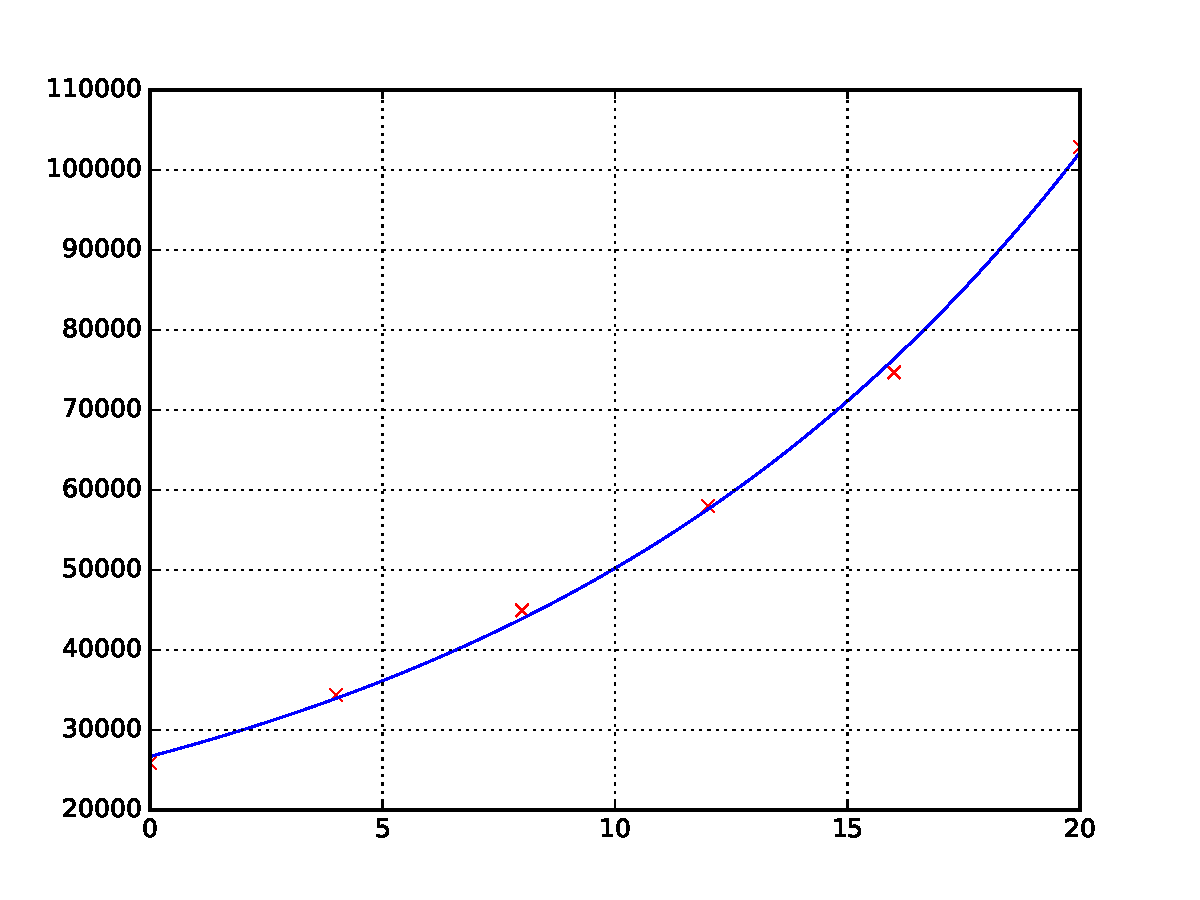
\includegraphics[width = 0.8\textwidth]{../Messdaten/plots/frequenzsweep_LC.pdf}
  \caption{LC-Kette, Gemessene Referenzwerte des Frequenzssweeps und exponentieller Fit}
  \label{fig: plot_sweep_LC}
\end{figure}
Auf analoge Weise sollen nun die beiden Grenzfrequenzen der $LC_1C_2$-Kette bestimmt werden. Die Referenzwerte
des Sweeps sind in Tabelle \ref{tab: sweep_LC1C2} einzusehen.
\FloatBarrier
\begin{table} 
\centering 
\caption{$LC_1C_2$-Kette, Referenzpunkte für den Frequenzsweep} 
\label{tab: sweep_LC1C2} 
\begin{tabular}{S S } 
\toprule  
{x in $\si{\centi\meter}$} & {Frequenzen in $\si{\hertz}$}  \\ 
\midrule  
 0  & 25608\\ 
4  & 34682\\ 
8  & 45788\\ 
12  & 58978\\ 
16  & 75244\\ 
20  & 104741\\ 
\bottomrule 
\end{tabular} 
\end{table}
Für die Fit-Parameter wurden folgende Werte berechnet:
\begin{align}
  \begin{aligned}
    A\ua{LC_1C_2} &= \SI{2.0(5)e4}{\hertz}\\
    B\ua{LC_1C_2} &= \SI{0.078(11)}{\cm^{-1}}\\
    C\ua{LC_1C_2} &= \SI{6(7)e3}{\hertz}
  \end{aligned}
  \label{eq: params_LC1C2}
\end{align}
Die Messwerte, sowie der Verlauf des Fits sind in Abbildung \ref{fig: plot_sweep_LC1C2} dargestellt.
Aus dem zur unteren Grenzfrequenz \eqref{eq: } gehörenden Abstand $x\ua{u} = \SI{6.5(5)}{\cm}$ ergibt sich die Frequenz:
\begin{equation}
  \nu\ua{G, u, exp} = \SI{4.0(12)e4}{\hertz}
\end{equation}
Die obere Grenzfrequenz \eqref{eq: } berechnet sich mit $x\ua{o} = \SI{10.7(5)}{\cm}$ zu:
\begin{equation}
    \nu\ua{G, o, exp} = \SI{5.3(15)e4}{\hertz}
\end{equation}
Hiermit können die mittleren prozentualen Abweichungen von den Theoriewerten bestimmt werden.
\begin{align}
  \nu\ua{G,u,th} &= \SI{3.63e4}{\hertz}\\
  d\ua{LC_1C_2,u} &= 11 \%\\
  \nu\ua{G,o,th} &= \SI{5.55e4}{\hertz}\\
  d\ua{LC_1C_2, o} &= 4 \%
\end{align}
\FloatBarrier
\begin{figure}
  \centering
  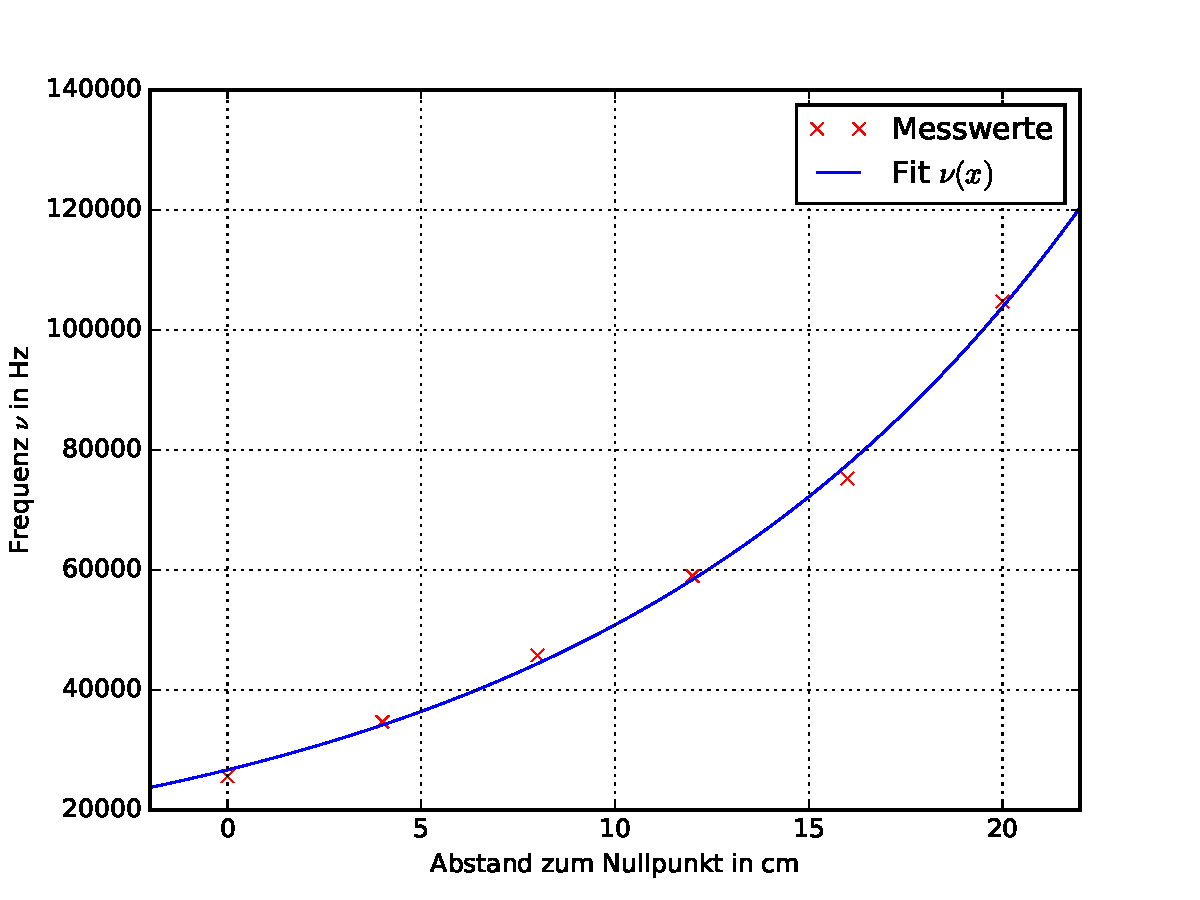
\includegraphics[width = 0.8\textwidth]{../Messdaten/plots/frequenzsweep_LC1C2.pdf}
  \caption{$LC_1C_2$-Kette, Gemessene Referenzwerte des Frequenzssweeps und exponentieller Fit}
  \label{fig: plot_sweep_LC1C2}
\end{figure}
\newpage
\subsection{Dispersionskurven}
Die gemäß \eqref{eq: } und \eqref{eq: } berechneten Dispersionskurven sind in den Abbildungen \ref{fig: dispersion_LC} und \ref{fig: dispersion_LC1C2}
dargestellt. Die gemessenen Frequenzen $\nu$ bei den Gesamtphasenverschiebungen, deren Betrag ein Vielfaches von $\pi$ beträgt,
sind in Tabelle \ref{tab: dispersion_LC} und \ref{tab: dispersion_LC1C2} aufgeführt. Hierbei wurde die Gesamtphasenverschiebung direkt durch die
Anzahl der Kettenglieder $n = 16$ geteilt, um die Phasenverschiebung pro Glied zu erhalten. Im Falle der $LC_1C_2$-Kette
wurden Ergebnisse mit $\theta > \pi/2$ so interpretiert, sodass sie gemäß der Periodizität der Funktion \eqref{eq: } im Intervall
$[0, \pi/2]$ liegen. Die Wertepaare wurden ebenfalls in den Abbildungen \ref{fig: dispersion_LC} und \ref{fig: dispersion_LC1C2} visualisiert.
\begin{table} 
\centering 
\caption{LC-Kette, Gemessene Frequenzen mit zugeordnetem Phasenversatz pro Glied} 
\label{tab: dispersion_LC} 
\begin{tabular}{S S } 
\toprule  
{$\theta$} & {$\nu$ in $\si{\hertz}$}  \\ 
\midrule  
 0.2  & 5022\\ 
0.4  & 10044\\ 
0.6  & 14811\\ 
0.8  & 19521\\ 
1.0  & 24211\\ 
1.2  & 28481\\ 
1.4  & 32477\\ 
1.6  & 36301\\ 
1.8  & 39777\\ 
2.0  & 42473\\ 
2.2  & 45084\\ 
2.4  & 47232\\ 
\bottomrule 
\end{tabular} 
\end{table}
\begin{table} 
\centering 
\caption{$LC_1C_2$-Kette, Gemessene Frequenzen mit zugeordnetem Phasenversatz pro Glied} 
\label{tab: dispersion_LC1C2} 
\begin{tabular}{S S } 
\toprule  
{$\theta$} & {$\nu$ in $\si{\hertz}$}  \\ 
\midrule  
 0.2  & 5776\\ 
0.4  & 11484\\ 
0.6  & 17187\\ 
0.8  & 22418\\ 
1.0  & 27092\\ 
1.2  & 31348\\ 
1.4  & 34736\\ 
1.6  & 55425\\ 
1.4  & 57163\\ 
1.2  & 59011\\ 
1.0  & 61105\\ 
0.8  & 63016\\ 
0.6  & 64572\\ 
\bottomrule 
\end{tabular} 
\end{table}

\begin{figure}
  \centering
  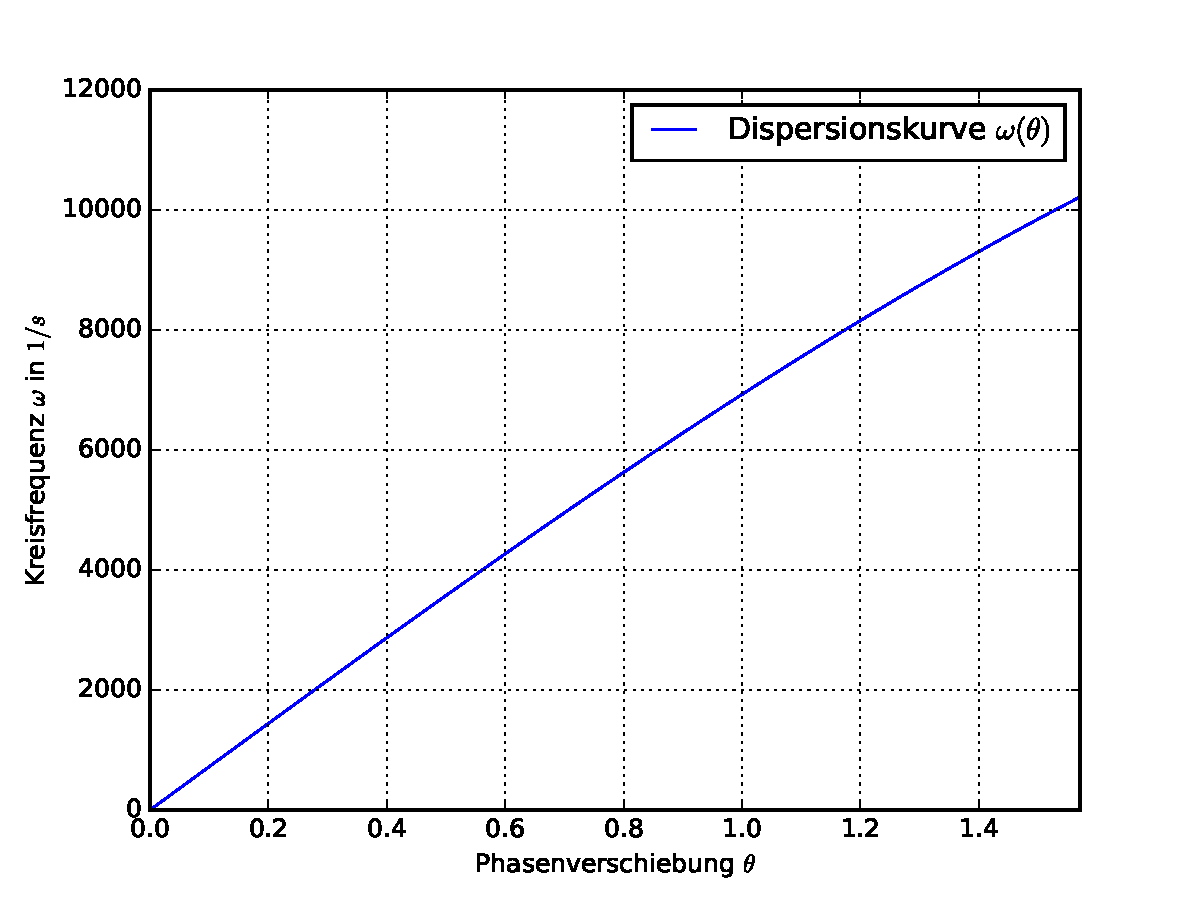
\includegraphics[width = 0.8\textwidth]{../Messdaten/plots/dispersion.pdf}
  \caption{LC-Kette, Verlauf der theoretischen Dispersionskurve und gemessene Werte}
  \label{fig: dispersion_LC}
\end{figure}
\begin{figure}
  \centering
  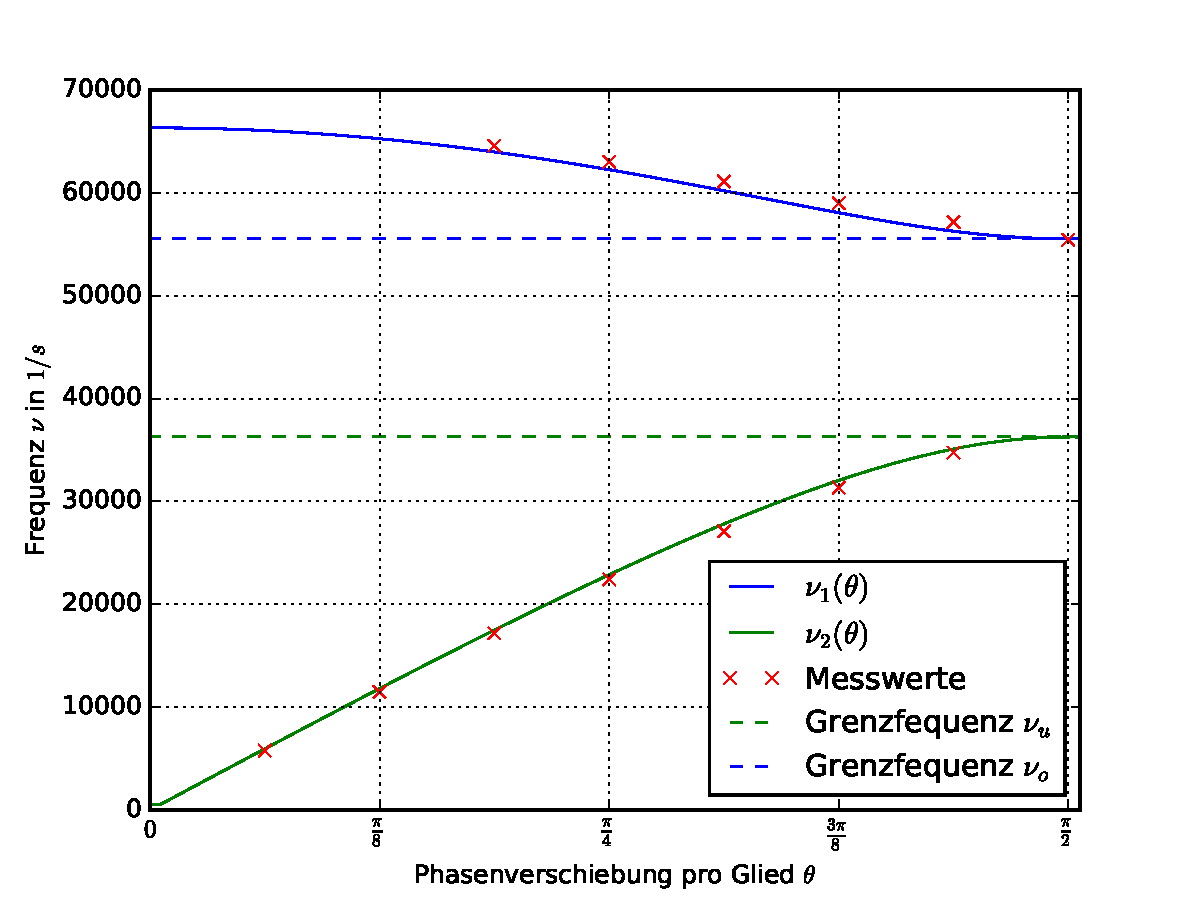
\includegraphics[width = 0.8\textwidth]{../Messdaten/plots/dispersion1.pdf}
  \caption{$LC_1C_2$-Kette, Verlauf der theoretischen Dispersionskurve und gemessene Werte}
  \label{fig: dispersion_LC1C2}
\end{figure}
\FloatBarrier


\subsection{Bestimmung der Phasengeschwindigkeit}
Die gemessenen Eigenfrequenzen, die die Spannung am Anfang bzw. Ende der beiderseits
offenen Kette maximal werden lassen, sind in Tabelle \ref{tab: v_phase} eingetragen. Analog zum
voran gegangenen Abschnitt wurden ihnen die Phasenverschiebungen pro Kettenglied $\theta$
zugeordnet. Aus dem Quotienten $\nu / \theta$ ergeben sich die Phasengeschwindigkeiten $v\ua{ph}$.
Die Wertepaare aus Phasengeschwindigkeit und zugehöriger Frequenz, sowie die gemäß \eqref{eq: } berechnete
Theoriekurve sind in Abbildung \ref{fig: v_phase} dargestellt.
\begin{table} 
\centering 
\caption{Eigenfrequenzen der LC Kette und berechnete Phasengeschwindigkeiten} 
\label{tab: v_phase} 
\begin{tabular}{S S S } 
\toprule  
{Phasenverschiebung $\theta$} & {Frequenzen in $\si{\hertz}$} & {$v_{ph}$ in $\si{\meter\per\second}$}  \\ 
\midrule  
 0  & 5092  & 162944\\ 
0  & 10004  & 160064\\ 
1  & 14770  & 157547\\ 
1  & 19741  & 157928\\ 
1  & 24062  & 153997\\ 
1  & 28625  & 152667\\ 
1  & 32446  & 148325\\ 
2  & 36468  & 145872\\ 
2  & 39235  & 139502\\ 
2  & 42527  & 136086\\ 
2  & 46630  & 135651\\ 
2  & 47523  & 126728\\ 
3  & 50052  & 123205\\ 
\bottomrule 
\end{tabular} 
\end{table}
\begin{figure}
  \centering
  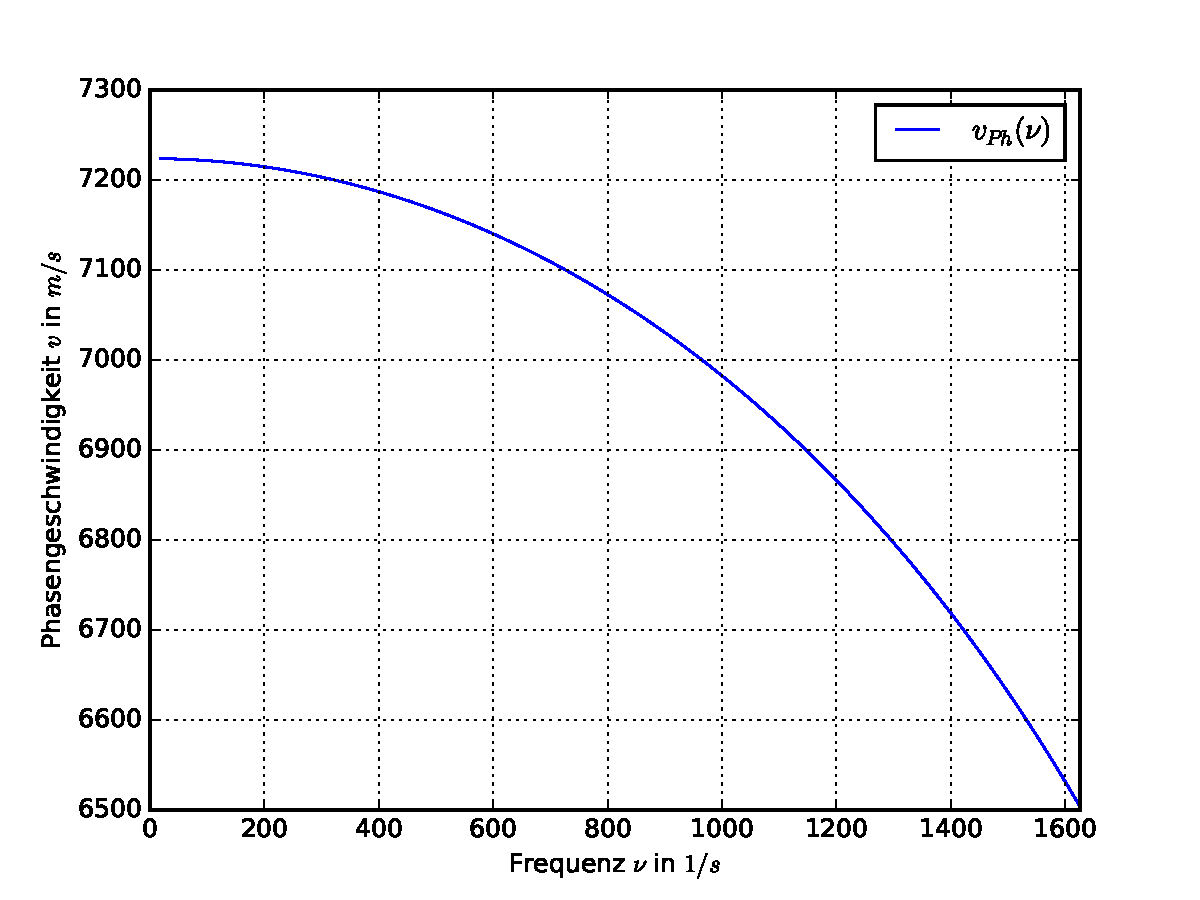
\includegraphics[width = 0.8\textwidth]{../Messdaten/plots/v_phase.pdf}
  \caption{Verlauf der Phasengeschwindigkeit in Relation zur Frequenz}
  \label{fig: v_phase}
\end{figure}


\subsection{Untersuchung stehender Wellen}
Für die ersten beiden Eigenfrequenzen $\nu_1 = \SI{5092}{\hertz}$ und $\nu_2 = \SI{10004}{\hertz}$ wurden
die Spannungsverläufe $U_{\nu_1}$ und $U_{\nu_2}$ der offenen LC-Kette entlang der einzelnen Kettenglieder vermessen. Die Messwerte sind in Tabelle
\ref{tab: U_nu12} einzusehen. Die Visualisierungen der einzelnen Verläufe befinden sich in den Abbildungen \ref{fig: U_nu1} und \ref{fig: U_nu2}.\par
\begin{table} 
\centering 
\caption{Spannungsverläufe $U_{\nu_1}$ und $U_{\nu_2}$ unter den Eigenfrequenzen $\nu_1$ und $\nu_2$ bei der offenen LC-Kette; Spannungsverlauf $U_{G}$ der geschlossenen LC-Kette} 
\label{tab: U_nu12} 
\begin{tabular}{S S S S } 
\toprule  
{Messpunkte} & {$U_{\nu_1}$ in $\si{\volt}$} & {$U_{\nu_2}$ in $\si{\volt}$} & {$U_{G}$ in $\si{\volt}$ }  \\ 
\midrule  
 1  & 1.80  & 2.20  & 0.41\\ 
2  & 1.75  & 2.05  & 0.41\\ 
3  & 1.65  & 1.55  & 0.41\\ 
4  & 1.50  & 0.80  & 0.42\\ 
5  & 1.25  & 0.00  & 0.43\\ 
6  & 0.95  & 0.85  & 0.44\\ 
7  & 0.65  & 1.55  & 0.44\\ 
8  & 0.30  & 2.05  & 0.43\\ 
9  & 0.10  & 2.25  & 0.42\\ 
10  & 0.40  & 2.05  & 0.41\\ 
11  & 0.75  & 1.55  & 0.41\\ 
12  & 1.05  & 0.85  & 0.41\\ 
13  & 1.35  & 0.00  & 0.42\\ 
14  & 1.55  & 0.85  & 0.42\\ 
15  & 1.70  & 1.60  & 0.43\\ 
16  & 1.80  & 2.10  & 0.44\\ 
17  & 1.80  & 2.25  & 0.43\\ 
\bottomrule 
\end{tabular} 
\end{table}
\begin{figure}
  \centering
  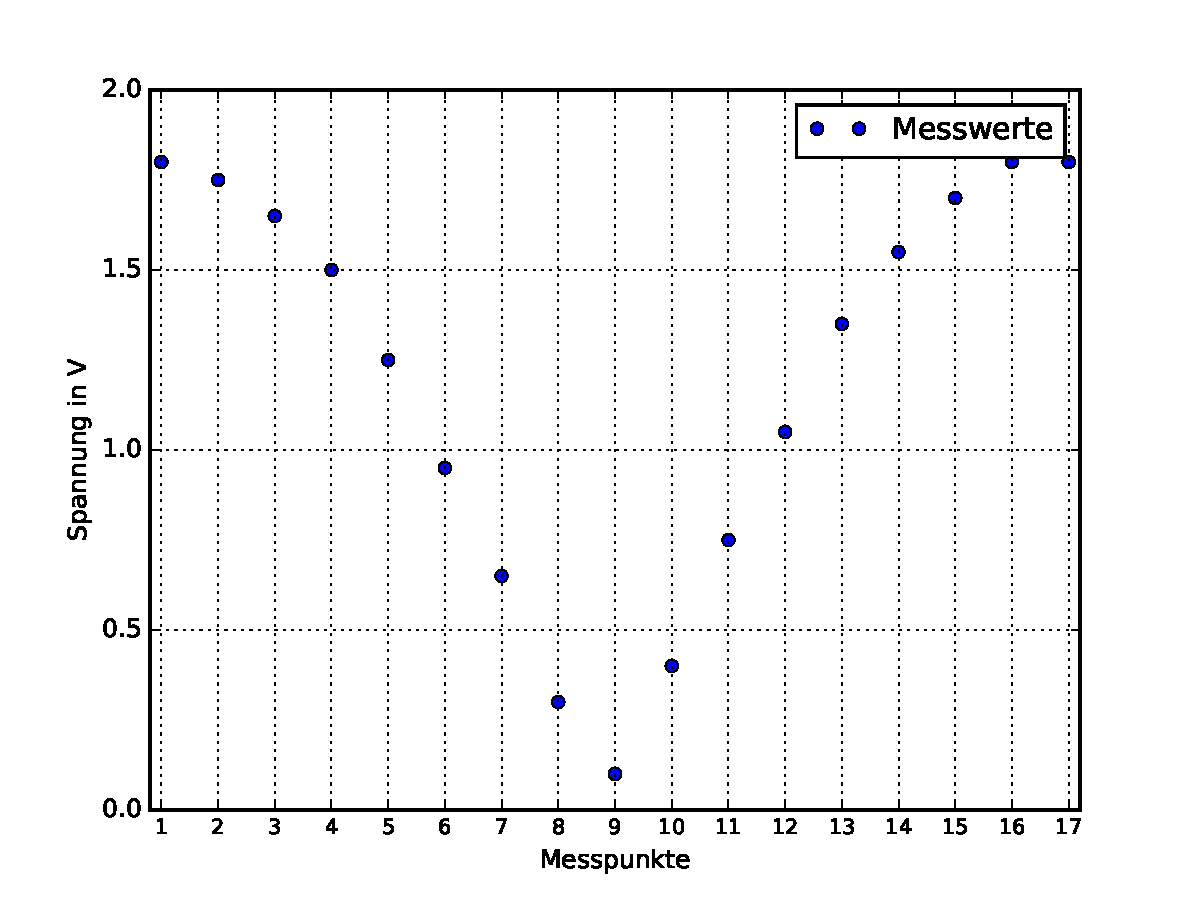
\includegraphics[width = 0.8\textwidth]{../Messdaten/plots/spannungsverlauf_nu1.pdf}
  \caption{Verlauf der Spannung entlang der offenen LC-Kette unter der Frequenz $\nu_1$}
  \label{fig: U_nu1}
\end{figure}
\begin{figure}
  \centering
  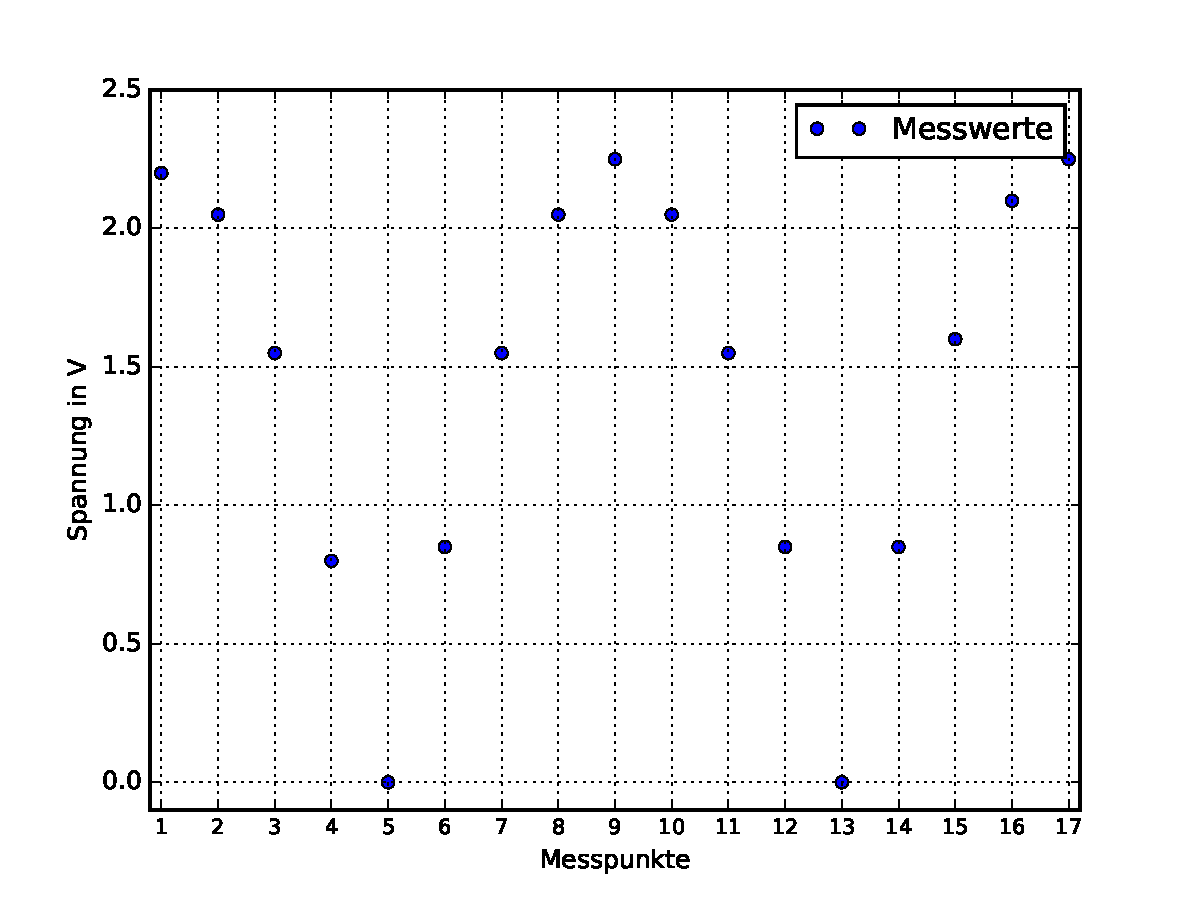
\includegraphics[width = 0.8\textwidth]{../Messdaten/plots/spannungsverlauf_nu2.pdf}
  \caption{Verlauf der Spannung entlang der offenen LC-Kette unter der Frequenz $\nu_2$}
  \label{fig: U_nu2}
\end{figure}
Bei der Frequenz $\nu\ua{G} = \SI{7762}{\hertz}$ wurde der Verlauf der Spannung der geschlossenen LC-Kette untersucht. Der Wellenwiderstand
wurde gemäß \eqref{eq: } berechnet. Für die Frequenz $\omega = 0$ ergibt sich der Wert $Z(0) = \SI{282.04}{\ohm}$. Die entlang der Kette gemessenen
Spannungen $U\ua{G}$ sind ebenfalls in Tabelle \ref{tab: U_nu12} aufgetragen. Ein Diagramm der Werte findet sich in Abbildung \ref{fig: U_G}
\begin{figure}
  \centering
  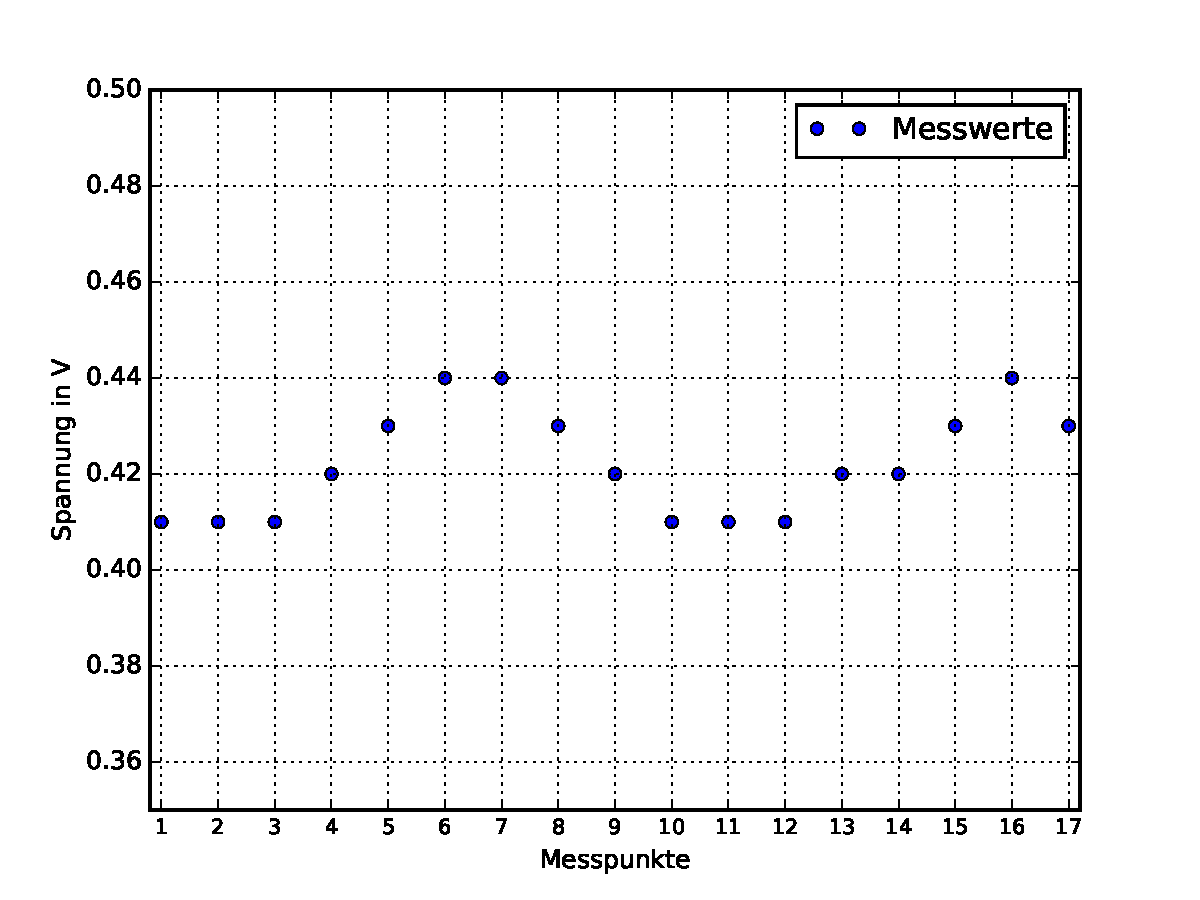
\includegraphics[width = 0.8\textwidth]{../Messdaten/plots/spannungsverlauf_geschlossen.pdf}
  \caption{Verlauf der Spannung entlang der geschlossenen LC-Kette unter der Frequenz $\nu_G$}
  \label{fig: U_G}
\end{figure}
